








\begin{figure*}[t]
    \centering
    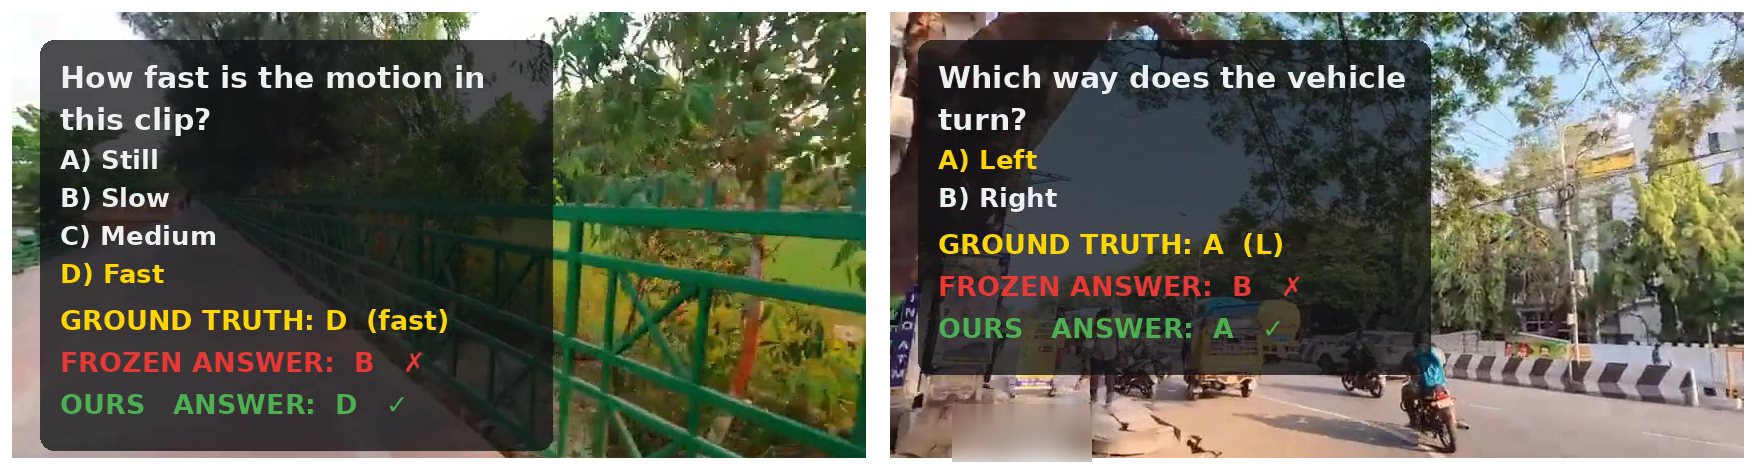
\includegraphics[width=\textwidth]{figures/demo_cards_teaser.png}
    \caption{\textbf{Same question, two encoders.} Each held-out clip is posed as a multiple-choice question with a ground-truth answer, then answered twice from an identical attentive probe head: once over the \textbf{frozen} V-JEPA~2.1 encoder and once over \textbf{ours} (factor-view predictor surgery). Only the backbone differs. \emph{Left:} motion-speed quartile from optical flow (ours 69.8\% vs frozen 60.9\% over 1{,}825 held-out clips; chance 25.6\%). \emph{Right:} vehicle turn direction under a leave-one-video-out split. Selected qualitative examples.}
    \label{fig:demo_cards}
    \vspace{-1.0em}
\end{figure*}

\begin{figure*}[t]
    \centering
    
\includegraphics[width=\textwidth]{figures/denseworld_scene_types_overview.png}
    \caption{\textbf{DENSEWORLD 1.0 scene-type coverage.}
    Representative examples from the dataset illustrate the breadth of urban environments covered by \textbf{DENSEWORLD 1.0}, including \textbf{market}, \textbf{residential}, \textbf{commercial}, \textbf{promenade}, \textbf{transit}, \textbf{highway}, \textbf{heritage}, \textbf{junction}, \textbf{flyover}, \textbf{beach}, \textbf{ghat}, \textbf{bazaar}, and \textbf{skyline} scenes. This diversity reflects the spatial, social, and infrastructural heterogeneity of populous, crowded, and chaotic Global South urban environments.}
    \label{fig:denseworld_scene_types}
    \vspace{-1.5em}
\end{figure*}















































































